\section{\wasm overview}
\label{sota:wasm}

%\renewcommand{\lstnumberautorefname}{Line}
\newcommand{\lstnumberautorefname}{Line}
\newcommand{\lineref}[1]{\autoref{#1}}


%\todo{Intro}

%\subsection*{}

% Javascript was first, and then more attempts.
Over the past decades, JavaScript has been used in the majority of the browser clients to allow client-side scripting. However, due to the complexity of this language and to gain in performance, several approaches appeared, supporting different languages in the browser.  For example, Java applets were introduced on web pages late in the 90's, Microsoft made an attempt with ActiveX in 1996  and Adobe added ActionScript later on 1998. All these attempts failed to persist, mainly due to security issues and the lack of consensus on the community of browser vendors. 

% asm.js and the demonstration of bad language patterns
In 2014, Emscripten proposed with a strict subset of JavaScript, asm.js, to allow low level code such as C to be compiled to JavaScript itself. Asm.js was first implemented as an LLVM backend. This approach came with the benefits of having all the ahead-of-time optimizations from LLVM, gaining in performance on browser clients \cite{asmjs} compared to standard JavaScript code. The main reason why asm.js is faster, is that it limits the language features to those that can be optimized in the LLVM pipeline or those that can be directly translated from the source code. Besides, it removes the majority of the dynamic characteristics of the language, limiting it to numerical types, top-level functions, and one large array in the memory directly accessed as raw data. Since asm.js is a subset of JavaScript it was compatible with all engines at that moment. Asm.js demonstrated that client-code could be improved with the right language design and standarization.
% Limitations o0f asm.js and the birth of Wasm
The work of Van Es \etal \cite{EsAsm.js} proposed to shrink JavaScript to asm.js in a source-to-source strategy, closing the cycle and extending the fact that asm.js was mainly a compilation target for C/C++ code. Despite encouraging results, JavaScript faces several limitations related to the characteristics of the language. For example, any JavaScript engine requires the parsing and the recompilation of the JavaScript code which implies significant overhead.

Following the asm.js initiative, the W3C publicly announced the \wasm (Wasm) language in 2015. \wasm is a binary instruction format for a stack-based virtual machine and was officially stated later by the work of Haas \etal \cite{Haas_2017} in 2017. The announcement of \wasm marked the first step of standarizing bytecode in the web environment. Wasm is designed to be fast, portable, self-contained and secure, and it outperforms asm.js \cite{Haas_2017}. Since 2017, the adoption of \wasm keeps growing. For example; Adobe, announced a full online version of Photoshop\footnote{\url{https://twitter.com/Adobe/status/1453034805004685313?s=20&t=Zf1N7-WmzecA0K4V8R69lw}} written in WebAssembly;  game companies moved their development from JavaScript to Wasm like is the case of a full Minecraft version \footnote{\url{https://satoshinm.github.io/NetCraft/}}; and the case of Blazor \footnote{\url{https://dotnet.microsoft.com/en-us/apps/aspnet/web-apps/blazor}}, a .Net virtual machine implemented in Wasm, able to execute C\# code in the browser.

%\todo{Benchmarks}

\subsection*{From source to Wasm}

All \wasm programs are compiled ahead-of-time from source languages. LLVM includes Wasm as a backend since version 8.0.0, supporting a broad range of frontend languages such as C/C++, Rust, Go or AssemblyScript\footnote{subset of the TypeScript language}. The resulting binary, works similarly to a traditional shared library, it includes instruction codes, symbols and exported functions. In \autoref{diagrams:sota:wasm}, we illustrate the workflow from the creation of Wasm binaries to their execution in the browser. The process starts by compiling the source code program to Wasm (Step \step{1}). This step includes ahead-of-time optimizations. For example, if the Wasm binary is generated out of the LLVM pipeline, all optimizations in the LLVM 

%To the best of our knowledge, the most complete survey about Wasm tooling is presented in the Awesome Wasm (\url{https://github.com/mbasso/awesome-wasm}) repo. It is a cumulative GitHub repo which includes references to articles, papers, books, demos, compilers and engines related to \wasm. 

The step \step{2} builds the standard library for Wasm usually as JavaScript code. This code includes the external functions that the Wasm binary needs for its execution inside the host engine. For example, the functions to interact with the DOM of the HTML page are imported in the Wasm binary during its call from the JavaScript code. The standard library can be manually written, however, compilers like Emscripten, Rust and Binaryen can generate it automatically, making this process completely transparent to developers.

Finally, the third step (Step \step{3}), includes the compilation and execution of the client-side code. Most of the browser engines compile either the Wasm and JavaScript codes to machine code. In the case of JavaScript, this process involves JIT and hot code replacement during runtime. For Wasm, since it is closer to machine code and it is already optimized, this process is a one-to-one mapping. For instance, in the case of V8, the compilation process only applies simple and fast optimizations such as constant folding and dead code removal. Once V8 completes the compilation process, the generated machine code for Wasm is final and is the same used along all its executions. This analysis was validated by conversations with the V8's dev team and by experimental studies in our previous contributions.  

\begin{figure}[h]
    \centering
    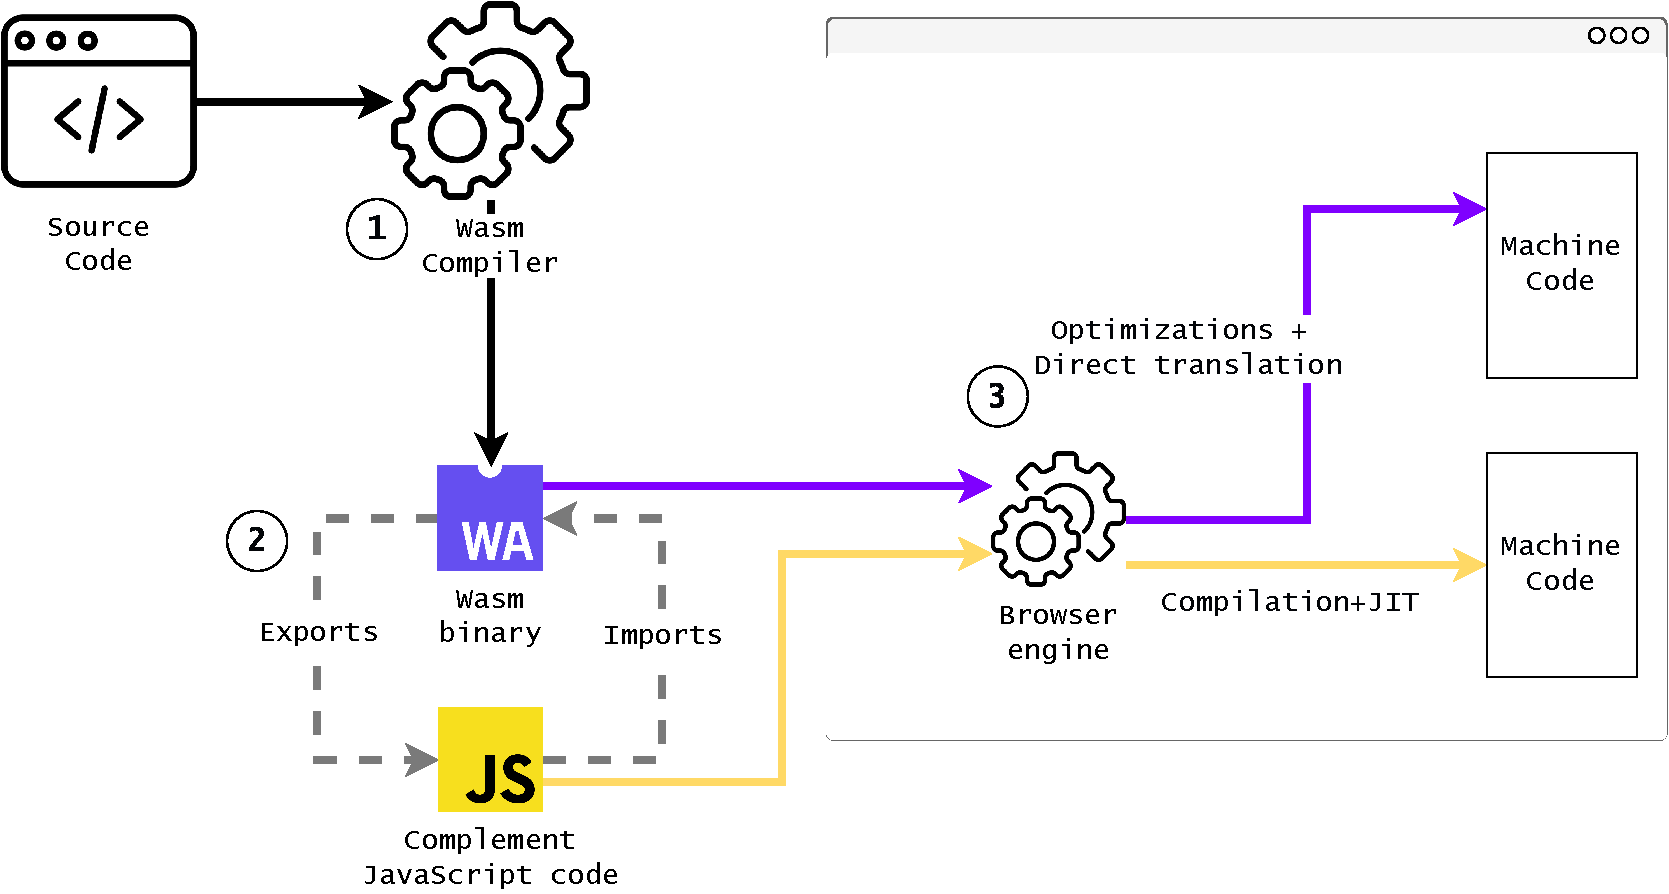
\includegraphics[width=\linewidth]{diagrams/wasm_workflow.pdf}
    \caption{WebAssembly building, compilation in the host engine and execution. }
    \label{diagrams:sota:wasm}
\end{figure}

Wasm can execute directly and is platform independent, making it useful for IoT and Edge computing \cite{Narayan2021Swivel,Sledge}. For instance, Cloudflare and Fastly adapted their platforms to provide Function as a Service (FaaS) directly with \wasm. In this case, the standard library, instead of JavaScript, is provided by any other language stack that the host environment supports.
In 2019, the Bytecode Alliance \footnote{\url{https://bytecodealliance.org/}} proposed WebAssembly System Interface (WASI) \cite{WASI}. WASI is the foundation to build Wasm code outside of the browser with a POSIX system interface platform. It standarizes the adoption of \wasm outside web browsers \cite{bryant2020webassembly} in heterogeneous platforms. 

% Talk about benchmarks and performance numbers

%Previous studies resulted in performance increasing in terms of bandwidth saving, execution, and process-on-demand spawning \cite{9640153, wen2020wasmachine}. The words of Solomon Hykes \footnote{\url{https://twitter.com/solomonstre/status/1111004913222324225}}, the former CEO of docker, show the impact of WASI: 

%\begin{displayquote}
%\textit{
%    If WASM+WASI existed in 2008, we wouldn't have needed to created Docker. That's how important it is. Webassembly on the server is the future of computing. A standardized system interface was the missing link. Let's hope WASI is up to the task!
%}
%\end{displayquote}

%\todo{How to obtain WebAssembly binaries}

%\todo{Browser workflow}

%\todo{How interpreters work, explain the workflow of V8 as it was validated by the V8 compiler developers}

%\todo{Backend workflow}

%\todo{Add a table with tools and interpreters: V8, SpiderMonkey, wasmtime, wasmer, sledge, warduino }


\subsection*{WebAssembly specificities}

% General description and the introduction of the component, module and section terms
\wasm defines its own Instruction Set Architecture (ISA) \cite{wasm_spec}. It is an abstraction close to machine code instructions but agnostic to CPU architectures. Thus, Wasm is platform independent. The ISA of Wasm includes also the necessary components that the binary requires to run in any host engine. 
A Wasm binary has a unique module as its main component. A module is composed by sections, corresponding to 13 types, each of them with an explicit semantic and a specific order inside the module. This makes the compilation to machine code faster. %The binary format of Wasm can include custom sections. For example, the work of \todo{Doe} proposed the usage of custom sections to sign binaries for the sake of trusting. 


% Example and intro to the stack
In \autoref{CExample} and \autoref{WASMExample} we illustrate a C program and its compilation to Wasm. The C function contains: heap allocation, external function declaration and the definition of a function with a loop, conditional branching, function calls and memory accesses. The code in \autoref{WASMExample} is in the textual format for the generated Wasm. The module in this case first defines the signature of the functions(\lineref{tpe1}, \lineref{tpe2}  and  \lineref{tpe3})  that help in the validation of the binary defining its parameter and result types. The information exchange between the host and the Wasm binary might be in two ways, exporting and importing functions, memory and globals to and from the host engine (\lineref{import1}, \lineref{export1} and \lineref{export2}). The definition of the function (\lineref{func1}) and its body follows the last import declaration at \lineref{import1}. 

% Functions
The function body is composed by local variable declarations and typed instructions that are evaluated in a virtual stack (Line 7 to Line 32 in \autoref{WASMExample}). Each instruction reads its operands from the stack and pushes back the result. The result of a function call is the top value of the stack at the end of the execution. In the case of \autoref{WASMExample}, the result value of the main function is the calculation of the last instruction, \texttt{i32.add} at \lineref{result}. A valid Wasm binary should have a valid stack structure that is verified during its translation to machine code. The stack validation is carried out using the static types of Wasm, \texttt{i32}, \texttt{i64}, \texttt{f32} and \texttt{f64}. As the listing shows, instructions are annotated with a numeric type.

% Example
\begin{code}
    \begin{minipage}[t]{0.4\linewidth}
        \lstset{language=C,caption={Example C function.},
        label=CExample,
        basicstyle=\small\ttfamily,
        escapeinside={(*@}{@*)}
        }
\input{sota/code/code.c}
\end{minipage}\hspace{10mm}
\begin{minipage}[t]{0.4\linewidth}
\lstset{
    language=WAT,
    caption={\wasm code  for \autoref{CExample}.},
    style=WATStyle,
    %stepnumber=0,
    escapeinside={(*@}{@*)},
    numbers=left,
    label=WASMExample}

%
\input{sota/code/code.fix.wat}
%\end{lstlisting}
\end{minipage}


%\begin{tikzpicture}[remember picture,overlay]

%\path (2.west) edge[<-, black] (1.west);
%\path (3.west) edge[<-,  black] (4.west);

%\path (6.east) edge[<-, bend right, black] (3.east);
%\path (9.east) edge[<-, bend right, black] (4.east);
%\path (7.east) edge[<-, bend right, black] (8.east);


%\end{tikzpicture}
\end{code}

% Memory, globals and functions
Wasm manages the memory in a restricted way.A Wasm module has a linear memory component that is accessed as \texttt{i32} pointers and should be isolated from the virtual stack. The declaration of the linear data in the memory is showed in \lineref{data}. The memory access is illustrated in \lineref{load}. This memory is usually bound in browser engines to 2Gb of size, and it is only shareable between the process that instantiate the Wasm binary and the binary itself (explicitly declared in \lineref{mem1} and \lineref{export2}). Therefore, this ensures the isolation of the execution of Wasm code. 

Wasm also provides global variables in their four primitive types. Global variables (\lineref{global1}) are only accessible by their declaration index, and it is not possible to dynamically address them. For functions, Wasm follows the same mechanism, either the functions are called by their index (\lineref{call}) or using a static table of function declarations. This latter allows modeling dynamic calls of functions (through pointers) from languages such as C/C++; however, the compiler should populate the static table of functions.


In Wasm, all instructions are grouped into blocks, being the start of a function the root block. Two consecutive block declarations can be appreciated in \lineref{block1} and \lineref{block2} of \autoref{WASMExample}. Control flow structures jump between block boundaries and not to any position in the code like regular assembly code. A block may specify the state that the stack must have before its execution and the result stack value coming from its instructions. Inside the Wasm binary the blocks explicitly define where they start and end (\lineref{end1} and \lineref{end2}). By design, each block executes independently and cannot execute or refer to outer block values. This is quarantieed by explicitly annotating the state of the stack before and after the block. Three instructions handle the navigation between blocks: unconditional break, conditional break (\lineref{break1} and \lineref{break2}) and table break. Each break instruction can only jump to one of its enclosing blocks. For example, in \autoref{WASMExample}, \lineref{break1} forces the execution to jump to the end of the first block at \lineref{block1} if the value at the top of the stack is greater than zero.

We want to remark that de description of Wasm in this section follows the version 1.0 of the language and not its proposals for extended features. We follow those features implemented in the majority of the vendors according to the Wasm roadmap \cite{wasm_roadmap}. On the other hand we excluded instructions for datatype conversion, table accesses and the majority of the arithmetic instructions for the sake of simplicity.

%There are two types of blocks, regular blocks, used to compound pieces of code for stack validation and loops. A loop block manages iterations, the only difference between this to blocks is that the breaking instruction jumps to the end of the block in the case of loops.

% Self contained loops

% Bound memory, no direct access to the DOM

% Roadmap: threads, SIMD, etc

%\todo{Wasm Semantics: Add a code listing, explain General layout of a binary, Function and signature, Instructions, Control flow, Memory model, Global model, table model}

%\todo{Add some sentences from the roadmap}

%\todo{Exported function signature allows typing validation before the code is executed}


\subsection*{WebAssembly's security}

As we described, \wasm is deterministic and well-typed, follows a structured control flow and explicitly separates its linear memory model, global variables and the execution stack. This design is robust \cite{WebAssemblySecurity} and makes easy for compilers and engines to sandbox the execution of Wasm binaries. Following the specification of Wasm for typing, memory, virtual stack and function calling,
host environments should provide protection against data corruption, code injection, and return-oriented programming (ROP).

However, WebAssembly is vulnerable under certain conditions, at the execution engine's level \cite{ChromeZero}.
Implementations in both browsers and standalone runtimes~\cite{Narayan2021Swivel} are vulnerable.
Genkin \etal demonstrated that Wasm could be used to exfiltrate data using cache timing-side channels \cite{Genkin2018DrivebyKC}.
One of our previous contributions trigger a CVE\footnote{\url{https://www.fastly.com/blog/defense-in-depth-stopping-a-wasm-compiler-bug-before-it-became-a-problem}} on the code generation component of wasmtime, highlighting that even when the language specification is meant to be secure, the underlying host implementation might not be. 
Moreover, binaries itself can be vulnerable. The work of Lehmann \etal ~\cite{usenixWasm2020} proved that C/C++ source code vulnerabilities can propagate to Wasm such as overwriting constant data or manipulating the heap using stackoverflow. Even though these vulnerabilities need a specific standard library implementation to be exploited, they make a call for better defenses for \wasm. 
% Current proposals
Several proposals for extending \wasm in the current roadmap could address some existing vulnerabilities. For example, having multiple memories could incorporate more than one memory, stack and global spaces, shrinking the attack surface. However, the implementation, adoption and settlement of the proposals are far from being a reality in all browser vendors.

% In fact, according to the work of Hilbig \etal \cite{Hilbig2021AnES}, the artificial variants created with one of our works contribute to the half of executable and available \wasm binaries in the wild.
